\documentclass[oneside, a4paper,11pt]{book}
\usepackage[margin=1in]{geometry}

\usepackage{graphicx}
\usepackage[utf8]{inputenc} % allow utf-8 input
\usepackage[T1]{fontenc}    % use 8-bit T1 fonts
\usepackage{hyperref}       % hyperlinks
\usepackage{url}            % simple URL typesetting
\usepackage{booktabs}       % professional-quality tables
\usepackage{nicefrac}       % compact symbols for 1/2, etc.
\usepackage{microtype}      % microtypography

\usepackage{listings}
\usepackage{xcolor}
\definecolor{codegreen}{rgb}{0,0.6,0}
\definecolor{codegray}{rgb}{0.5,0.5,0.5}
\definecolor{codepurple}{rgb}{0.58,0,0.82}
\definecolor{backcolour}{rgb}{0.95,0.95,0.92}

\lstdefinestyle{mystyle}{
    backgroundcolor=\color{backcolour},
    commentstyle=\color{codegreen},
    keywordstyle=\color{magenta},
    numberstyle=\tiny\color{codegray},
    stringstyle=\color{codepurple},
    basicstyle=\ttfamily\footnotesize,
    breakatwhitespace=false,
    breaklines=true,
    captionpos=b,
    keepspaces=true,
    numbers=left,
    numbersep=5pt,
    showspaces=false,
    showstringspaces=false,
    showtabs=false,
    tabsize=2
}
\lstset{style=mystyle}


\usepackage[autostyle]{csquotes}
\usepackage{dsfont}

\usepackage{algorithm,algpseudocode}
% \usepackage[ruled,vlined]{algorithm2e}
\usepackage{multicol}

\usepackage{hyperref}
\usepackage{amssymb}

\setlength{\parindent}{0pt}
\setlength{\parskip}{1em}

\newtheorem{theorem}{Theorem}
\newtheorem{definition}{Definition}
\newtheorem{proposition}{Proposition}
\newtheorem{corollary}{Corollary}

\newcommand\scalemath[2]{\scalebox{#1}{\mbox{\ensuremath{\displaystyle #2}}}}

\newcommand{\cyan}[1]{\textcolor{cyan}{#1}}

%%%%% NEW MATH DEFINITIONS %%%%%
\usepackage{amsmath,amsfonts,bm}
\usepackage{xspace}
\usepackage[nameinlink]{cleveref}


\crefformat{section}{\S#2#1#3} % see manual of cleveref, section 8.2.1
\crefname{algorithm}{Alg.}{Algs.}
\crefformat{subsection}{\S#2#1#3}
\Crefname{equation}{Eq.}{Eqs.}
\Crefname{figure}{Fig.}{Figs.}

%% abbr 
\newcommand{\ie}{{\em i.e.,}\xspace}
\newcommand{\cf}{{\em c.f.,}\xspace}
\newcommand{\eg}{{\em e.g.,}\xspace}
\newcommand{\etal}{{\em et al.,}\xspace}
\newcommand{\wrt}{\emph{w.r.t.}\xspace}
\newcommand{\aka}{\emph{a.k.a.}\xspace}
\newcommand{\resp}{\emph{resp.}\xspace}


\newcommand{\pos}{${pos}$}


%%% inline lists
\newcommand{\Ni}{({\em i})~}
\newcommand{\Nii}{({\em ii})~}
\newcommand{\Niii}{({\em iii})~}
\newcommand{\Niv}{({\em iv})~}
\newcommand{\Nv}{({\em v})~}
\newcommand{\Na}{({\em a})~}
\newcommand{\Nb}{({\em b})~}
\newcommand{\Nc}{({\em c})~}
\newcommand{\Nd}{({\em d})~}
\newcommand{\Ne}{({\em e})~}
\newcommand{\Nf}{({\em f})~}


\newcommand{\comm}[1]{\textcolor{blue}{\noindent #1}}
\newcommand{\alert}[1]{\textcolor{red}{\noindent$\Rightarrow$ #1}}
\newcommand{\red}[1]{\textcolor{red}{#1}}
\newcommand{\blue}[1]{\textcolor{blue}{#1}}
\newcommand{\magenta}[1]{\textcolor{magenta}{#1}}
\newcommand{\green}[1]{\textcolor{green}{#1}}
\newcommand{\teal}[1]{\textcolor{teal}{#1}}
\newcommand{\add}[1]{\textcolor{black}{#1}}

%\usepackage{amsmath,amsfonts,bm}
%\usepackage[tbtags]{amsmath}

% Mark sections of captions for referring to divisions of figures
\newcommand{\figleft}{{\em (Left)}}
\newcommand{\figcenter}{{\em (Center)}}
\newcommand{\figright}{{\em (Right)}}
\newcommand{\figtop}{{\em (Top)}}
\newcommand{\figbottom}{{\em (Bottom)}}
\newcommand{\captiona}{{\em (a)}}
\newcommand{\captionb}{{\em (b)}}
\newcommand{\captionc}{{\em (c)}}
\newcommand{\captiond}{{\em (d)}}


\newtheorem{prop}{Proposition}

\newcommand{\sarrow}[1][4pt]{\!\mathrel{%
   \vcenter{\hbox{\rule[-.5\fontdimen8\textfont3]{#1}{\fontdimen8\textfont3}}}%
   \mkern-4mu\hbox{\usefont{U}{lasy}{m}{n}\symbol{41}}}\!}
\makeatletter   
\newcommand{\sveryshortarrow}[1][3pt]{\mathrel{%
    \vcenter{\hbox{\rule[-.5\fontdimen8\scriptfont3]
               {\scriptratio\dimexpr#1\relax}{\fontdimen8\scriptfont3}}}%
   \mkern-4mu\hbox{\let\f@size\sf@size\usefont{U}{lasy}{m}{n}\symbol{41}}}}
\makeatother

% \newcommand{\sarrow}{{\veryshortarrow}}

\newtheorem{defi}{Definition}

% Highlight a newly defined term
\newcommand{\newterm}[1]{{\bf #1}}


% Figure reference, lower-case.
\def\figref#1{figure~\ref{#1}}
% Figure reference, capital. For start of sentence
\def\Figref#1{Figure~\ref{#1}}
\def\twofigref#1#2{figures \ref{#1} and \ref{#2}}
\def\quadfigref#1#2#3#4{figures \ref{#1}, \ref{#2}, \ref{#3} and \ref{#4}}
% Section reference, lower-case.
\def\secref#1{section~\ref{#1}}
% Section reference, capital.
\def\Secref#1{Section~\ref{#1}}
% Reference to two sections.
\def\twosecrefs#1#2{sections \ref{#1} and \ref{#2}}
% Reference to three sections.
\def\secrefs#1#2#3{sections \ref{#1}, \ref{#2} and \ref{#3}}
% Reference to an equation, lower-case.
\def\eqref#1{equation~\ref{#1}}
% Reference to an equation, upper case
\def\Eqref#1{Equation~\ref{#1}}
% A raw reference to an equation---avoid using if possible
\def\plaineqref#1{\ref{#1}}
% Reference to a chapter, lower-case.
\def\chapref#1{chapter~\ref{#1}}
% Reference to an equation, upper case.
\def\Chapref#1{Chapter~\ref{#1}}
% Reference to a range of chapters
\def\rangechapref#1#2{chapters\ref{#1}--\ref{#2}}
% Reference to an algorithm, lower-case.
\def\algref#1{algorithm~\ref{#1}}
% Reference to an algorithm, upper case.
\def\Algref#1{Algorithm~\ref{#1}}
\def\twoalgref#1#2{algorithms \ref{#1} and \ref{#2}}
\def\Twoalgref#1#2{Algorithms \ref{#1} and \ref{#2}}
% Reference to a part, lower case
\def\partref#1{part~\ref{#1}}
% Reference to a part, upper case
\def\Partref#1{Part~\ref{#1}}
\def\twopartref#1#2{parts \ref{#1} and \ref{#2}}

\def\ceil#1{\lceil #1 \rceil}
\def\floor#1{\lfloor #1 \rfloor}
\def\1{\bm{1}}
\newcommand{\train}{\mathcal{D}}
\newcommand{\valid}{\mathcal{D_{\mathrm{valid}}}}
\newcommand{\test}{\mathcal{D_{\mathrm{test}}}}

\def\eps{{\epsilon}}


% Random variables
\def\reta{{\textnormal{$\eta$}}}
\def\ra{{\textnormal{a}}}
\def\rb{{\textnormal{b}}}
\def\rc{{\textnormal{c}}}
\def\rd{{\textnormal{d}}}
\def\re{{\textnormal{e}}}
\def\rf{{\textnormal{f}}}
\def\rg{{\textnormal{g}}}
\def\rh{{\textnormal{h}}}
\def\ri{{\textnormal{i}}}
\def\rj{{\textnormal{j}}}
\def\rk{{\textnormal{k}}}
\def\rl{{\textnormal{l}}}
% rm is already a command, just don't name any random variables m
\def\rn{{\textnormal{n}}}
\def\ro{{\textnormal{o}}}
\def\rp{{\textnormal{p}}}
\def\rq{{\textnormal{q}}}
\def\rr{{\textnormal{r}}}
\def\rs{{\textnormal{s}}}
\def\rt{{\textnormal{t}}}
\def\ru{{\textnormal{u}}}
\def\rv{{\textnormal{v}}}
\def\rw{{\textnormal{w}}}
\def\rx{{\textnormal{x}}}
\def\ry{{\textnormal{y}}}
\def\rz{{\textnormal{z}}}

% Random vectors
\def\rvepsilon{{\mathbf{\epsilon}}}
\def\rvtheta{{\mathbf{\theta}}}
\def\rva{{\mathbf{a}}}
\def\rvb{{\mathbf{b}}}
\def\rvc{{\mathbf{c}}}
\def\rvd{{\mathbf{d}}}
\def\rve{{\mathbf{e}}}
\def\rvf{{\mathbf{f}}}
\def\rvg{{\mathbf{g}}}
\def\rvh{{\mathbf{h}}}
\def\rvu{{\mathbf{i}}}
\def\rvj{{\mathbf{j}}}
\def\rvk{{\mathbf{k}}}
\def\rvl{{\mathbf{l}}}
\def\rvm{{\mathbf{m}}}
\def\rvn{{\mathbf{n}}}
\def\rvo{{\mathbf{o}}}
\def\rvp{{\mathbf{p}}}
\def\rvq{{\mathbf{q}}}
\def\rvr{{\mathbf{r}}}
\def\rvs{{\mathbf{s}}}
\def\rvt{{\mathbf{t}}}
\def\rvu{{\mathbf{u}}}
\def\rvv{{\mathbf{v}}}
\def\rvw{{\mathbf{w}}}
\def\rvx{{\mathbf{x}}}
\def\rvy{{\mathbf{y}}}
\def\rvz{{\mathbf{z}}}

% Elements of random vectors
\def\erva{{\textnormal{a}}}
\def\ervb{{\textnormal{b}}}
\def\ervc{{\textnormal{c}}}
\def\ervd{{\textnormal{d}}}
\def\erve{{\textnormal{e}}}
\def\ervf{{\textnormal{f}}}
\def\ervg{{\textnormal{g}}}
\def\ervh{{\textnormal{h}}}
\def\ervi{{\textnormal{i}}}
\def\ervj{{\textnormal{j}}}
\def\ervk{{\textnormal{k}}}
\def\ervl{{\textnormal{l}}}
\def\ervm{{\textnormal{m}}}
\def\ervn{{\textnormal{n}}}
\def\ervo{{\textnormal{o}}}
\def\ervp{{\textnormal{p}}}
\def\ervq{{\textnormal{q}}}
\def\ervr{{\textnormal{r}}}
\def\ervs{{\textnormal{s}}}
\def\ervt{{\textnormal{t}}}
\def\ervu{{\textnormal{u}}}
\def\ervv{{\textnormal{v}}}
\def\ervw{{\textnormal{w}}}
\def\ervx{{\textnormal{x}}}
\def\ervy{{\textnormal{y}}}
\def\ervz{{\textnormal{z}}}

% Random matrices
\def\rmA{{\mathbf{A}}}
\def\rmB{{\mathbf{B}}}
\def\rmC{{\mathbf{C}}}
\def\rmD{{\mathbf{D}}}
\def\rmE{{\mathbf{E}}}
\def\rmF{{\mathbf{F}}}
\def\rmG{{\mathbf{G}}}
\def\rmH{{\mathbf{H}}}
\def\rmI{{\mathbf{I}}}
\def\rmJ{{\mathbf{J}}}
\def\rmK{{\mathbf{K}}}
\def\rmL{{\mathbf{L}}}
\def\rmM{{\mathbf{M}}}
\def\rmN{{\mathbf{N}}}
\def\rmO{{\mathbf{O}}}
\def\rmP{{\mathbf{P}}}
\def\rmQ{{\mathbf{Q}}}
\def\rmR{{\mathbf{R}}}
\def\rmS{{\mathbf{S}}}
\def\rmT{{\mathbf{T}}}
\def\rmU{{\mathbf{U}}}
\def\rmV{{\mathbf{V}}}
\def\rmW{{\mathbf{W}}}
\def\rmX{{\mathbf{X}}}
\def\rmY{{\mathbf{Y}}}
\def\rmZ{{\mathbf{Z}}}

% Elements of random matrices
\def\ermA{{\textnormal{A}}}
\def\ermB{{\textnormal{B}}}
\def\ermC{{\textnormal{C}}}
\def\ermD{{\textnormal{D}}}
\def\ermE{{\textnormal{E}}}
\def\ermF{{\textnormal{F}}}
\def\ermG{{\textnormal{G}}}
\def\ermH{{\textnormal{H}}}
\def\ermI{{\textnormal{I}}}
\def\ermJ{{\textnormal{J}}}
\def\ermK{{\textnormal{K}}}
\def\ermL{{\textnormal{L}}}
\def\ermM{{\textnormal{M}}}
\def\ermN{{\textnormal{N}}}
\def\ermO{{\textnormal{O}}}
\def\ermP{{\textnormal{P}}}
\def\ermQ{{\textnormal{Q}}}
\def\ermR{{\textnormal{R}}}
\def\ermS{{\textnormal{S}}}
\def\ermT{{\textnormal{T}}}
\def\ermU{{\textnormal{U}}}
\def\ermV{{\textnormal{V}}}
\def\ermW{{\textnormal{W}}}
\def\ermX{{\textnormal{X}}}
\def\ermY{{\textnormal{Y}}}
\def\ermZ{{\textnormal{Z}}}

% Vectors
\def\vzero{{\bm{0}}}
\def\vone{{\bm{1}}}
\def\vmu{{\bm{\mu}}}
\def\vtheta{{\bm{\theta}}}
\def\va{{\bm{a}}}
\def\vb{{\bm{b}}}
\def\vc{{\bm{c}}}
\def\vd{{\bm{d}}}
\def\ve{{\bm{e}}}
\def\vf{{\bm{f}}}
\def\vg{{\bm{g}}}
\def\vh{{\bm{h}}}
\def\vi{{\bm{i}}}
\def\vj{{\bm{j}}}
\def\vk{{\bm{k}}}
\def\vl{{\bm{l}}}
\def\vm{{\bm{m}}}
\def\vn{{\bm{n}}}
\def\vo{{\bm{o}}}
\def\vp{{\bm{p}}}
\def\vq{{\bm{q}}}
\def\vr{{\bm{r}}}
\def\vs{{\bm{s}}}
\def\vt{{\bm{t}}}
\def\vu{{\bm{u}}}
\def\vv{{\bm{v}}}
\def\vw{{\bm{w}}}
\def\vx{{\bm{x}}}
\def\vy{{\bm{y}}}
\def\vz{{\bm{z}}}

\def\vip{{\bm{i}\bm{p}}}

\def\vdelta{{\bm{\delta}}}
\def\valphaa{{\bm{\alpha}}}

% Elements of vectors
\def\evalpha{{\alpha}}
\def\evbeta{{\beta}}
\def\evepsilon{{\epsilon}}
\def\evlambda{{\lambda}}
\def\evomega{{\omega}}
\def\evmu{{\mu}}
\def\evpsi{{\psi}}
\def\evsigma{{\sigma}}
\def\evtheta{{\theta}}
\def\eva{{a}}
\def\evb{{b}}
\def\evc{{c}}
\def\evd{{d}}
\def\eve{{e}}
\def\evf{{f}}
\def\evg{{g}}
\def\evh{{h}}
\def\evi{{i}}
\def\evj{{j}}
\def\evk{{k}}
\def\evl{{l}}
\def\evm{{m}}
\def\evn{{n}}
\def\evo{{o}}
\def\evp{{p}}
\def\evq{{q}}
\def\evr{{r}}
\def\evs{{s}}
\def\evt{{t}}
\def\evu{{u}}
\def\evv{{v}}
\def\evw{{w}}
\def\evx{{x}}
\def\evy{{y}}
\def\evz{{z}}

% Matrix
\def\m1{{\bm{1}}}
\def\mA{{\bm{A}}}
\def\mB{{\bm{B}}}
\def\mC{{\bm{C}}}
\def\mD{{\bm{D}}}
\def\mE{{\bm{E}}}
\def\mF{{\bm{F}}}
\def\mG{{\bm{G}}}
\def\mH{{\bm{H}}}
\def\mI{{\bm{I}}}
\def\mJ{{\bm{J}}}
\def\mK{{\bm{K}}}
\def\mL{{\bm{L}}}
\def\mM{{\bm{M}}}
\def\mN{{\bm{N}}}
\def\mO{{\bm{O}}}
\def\mP{{\bm{P}}}
\def\mQ{{\bm{Q}}}
\def\mR{{\bm{R}}}
\def\mS{{\bm{S}}}
\def\mT{{\bm{T}}}
\def\mU{{\bm{U}}}
\def\mV{{\bm{V}}}
\def\mW{{\bm{W}}}
\def\mX{{\bm{X}}}
\def\mY{{\bm{Y}}}
\def\mZ{{\bm{Z}}}
\def\mBeta{{\bm{\beta}}}
\def\mPhi{{\bm{\Phi}}}
\def\mLambda{{\bm{\Lambda}}}
\def\mSigma{{\bm{\Sigma}}}

% Tensor
\DeclareMathAlphabet{\mathsfit}{\encodingdefault}{\sfdefault}{m}{sl}
\SetMathAlphabet{\mathsfit}{bold}{\encodingdefault}{\sfdefault}{bx}{n}

\newcommand{\tens}[1]{\bm{\mathsfit{#1}}}


\def\tA{{\tens{A}}}
\def\tB{{\tens{B}}}
\def\tC{{\tens{C}}}
\def\tD{{\tens{D}}}
\def\tE{{\tens{E}}}
\def\tF{{\tens{F}}}
\def\tG{{\tens{G}}}
\def\tH{{\tens{H}}}
\def\tI{{\tens{I}}}
\def\tJ{{\tens{J}}}
\def\tK{{\tens{K}}}
\def\tL{{\tens{L}}}
\def\tM{{\tens{M}}}
\def\tN{{\tens{N}}}
\def\tO{{\tens{O}}}
\def\tP{{\tens{P}}}
\def\tQ{{\tens{Q}}}
\def\tR{{\tens{R}}}
\def\tS{{\tens{S}}}
\def\tT{{\tens{T}}}
\def\tU{{\tens{U}}}
\def\tV{{\tens{V}}}
\def\tW{{\tens{W}}}
\def\tX{{\tens{X}}}
\def\tY{{\tens{Y}}}
\def\tZ{{\tens{Z}}}


% Graph
\def\gA{{\mathcal{A}}}
\def\gB{{\mathcal{B}}}
\def\gC{{\mathcal{C}}}
\def\gD{{\mathcal{D}}}
\def\gE{{\mathcal{E}}}
\def\gF{{\mathcal{F}}}
\def\gG{{\mathcal{G}}}
\def\gH{{\mathcal{H}}}
\def\gI{{\mathcal{I}}}
\def\gJ{{\mathcal{J}}}
\def\gK{{\mathcal{K}}}
\def\gL{{\mathcal{L}}}
\def\gM{{\mathcal{M}}}
\def\gN{{\mathcal{N}}}
\def\gO{{\mathcal{O}}}
\def\gP{{\mathcal{P}}}
\def\gQ{{\mathcal{Q}}}
\def\gR{{\mathcal{R}}}
\def\gS{{\mathcal{S}}}
\def\gT{{\mathcal{T}}}
\def\gU{{\mathcal{U}}}
\def\gV{{\mathcal{V}}}
\def\gW{{\mathcal{W}}}
\def\gX{{\mathcal{X}}}
\def\gY{{\mathcal{Y}}}
\def\gZ{{\mathcal{Z}}}
\def\gSP{{\mathcal{S}\mathcal{P}}}
\def\gLS{{\mathcal{L}\mathcal{S}}}
\def\gLU{{\mathcal{L}\mathcal{U}}}
\def\gST{{\mathcal{S}\mathcal{T}}}

% Sets
\def\sA{{\mathbb{A}}}
\def\sB{{\mathbb{B}}}
\def\sC{{\mathbb{C}}}
\def\sD{{\mathbb{D}}}
% Don't use a set called E, because this would be the same as our symbol
% for expectation.
\def\sF{{\mathbb{F}}}
\def\sG{{\mathbb{G}}}
\def\sH{{\mathbb{H}}}
\def\sI{{\mathbb{I}}}
\def\sJ{{\mathbb{J}}}
\def\sK{{\mathbb{K}}}
\def\sL{{\mathbb{L}}}
\def\sM{{\mathbb{M}}}
\def\sN{{\mathbb{N}}}
\def\sO{{\mathbb{O}}}
\def\sP{{\mathbb{P}}}
\def\sQ{{\mathbb{Q}}}
\def\sR{{\mathbb{R}}}
\def\sS{{\mathbb{S}}}
\def\sT{{\mathbb{T}}}
\def\sU{{\mathbb{U}}}
\def\sV{{\mathbb{V}}}
\def\sW{{\mathbb{W}}}
\def\sX{{\mathbb{X}}}
\def\sY{{\mathbb{Y}}}
\def\sZ{{\mathbb{Z}}}

\def\sSB{{\mathbb{S}\mathbb{B}}}

% Entries of a matrix
\def\emLambda{{\Lambda}}
\def\emA{{A}}
\def\emB{{B}}
\def\emC{{C}}
\def\emD{{D}}
\def\emE{{E}}
\def\emF{{F}}
\def\emG{{G}}
\def\emH{{H}}
\def\emI{{I}}
\def\emJ{{J}}
\def\emK{{K}}
\def\emL{{L}}
\def\emM{{M}}
\def\emN{{N}}
\def\emO{{O}}
\def\emP{{P}}
\def\emQ{{Q}}
\def\emR{{R}}
\def\emS{{S}}
\def\emT{{T}}
\def\emU{{U}}
\def\emV{{V}}
\def\emW{{W}}
\def\emX{{X}}
\def\emY{{Y}}
\def\emZ{{Z}}
\def\emSigma{{\Sigma}}

% entries of a tensor
% Same font as tensor, without \bm wrapper
\newcommand{\etens}[1]{\mathsfit{#1}}
\def\etLambda{{\etens{\Lambda}}}
\def\etA{{\etens{A}}}
\def\etB{{\etens{B}}}
\def\etC{{\etens{C}}}
\def\etD{{\etens{D}}}
\def\etE{{\etens{E}}}
\def\etF{{\etens{F}}}
\def\etG{{\etens{G}}}
\def\etH{{\etens{H}}}
\def\etI{{\etens{I}}}
\def\etJ{{\etens{J}}}
\def\etK{{\etens{K}}}
\def\etL{{\etens{L}}}
\def\etM{{\etens{M}}}
\def\etN{{\etens{N}}}
\def\etO{{\etens{O}}}
\def\etP{{\etens{P}}}
\def\etQ{{\etens{Q}}}
\def\etR{{\etens{R}}}
\def\etS{{\etens{S}}}
\def\etT{{\etens{T}}}
\def\etU{{\etens{U}}}
\def\etV{{\etens{V}}}
\def\etW{{\etens{W}}}
\def\etX{{\etens{X}}}
\def\etY{{\etens{Y}}}
\def\etZ{{\etens{Z}}}

% The true underlying data generating distribution
\newcommand{\pdata}{p_{\rm{data}}}
% The empirical distribution defined by the training set
\newcommand{\ptrain}{\hat{p}_{\rm{data}}}
\newcommand{\Ptrain}{\hat{P}_{\rm{data}}}
% The model distribution
\newcommand{\pmodel}{p_{\rm{model}}}
\newcommand{\Pmodel}{P_{\rm{model}}}
\newcommand{\ptildemodel}{\tilde{p}_{\rm{model}}}
% Stochastic autoencoder distributions
\newcommand{\pencode}{p_{\rm{encoder}}}
\newcommand{\pdecode}{p_{\rm{decoder}}}
\newcommand{\precons}{p_{\rm{reconstruct}}}

\newcommand{\laplace}{\mathrm{Laplace}} % Laplace distribution

\newcommand{\E}{\mathbb{E}}
\newcommand{\Ls}{\mathcal{L}}
\newcommand{\R}{\mathbb{R}}
\newcommand{\emp}{\tilde{p}}
\newcommand{\lr}{\alpha}
\newcommand{\reg}{\lambda}
\newcommand{\rect}{\mathrm{rectifier}}
\newcommand{\softmax}{\mathrm{softmax}}
%\newcommand{\softmax}{\mathcal{S}}


\newcommand{\ptr}{\rho}
\newcommand{\bptr}{bp}
\newcommand{\sptr}{sp}
\newcommand{\gptr}{gp}
%\newcommand{\lc}{lc}
\newcommand{\blb}{uc}
\newcommand{\glb}{gc}



\newcommand{\sigmoid}{\sigma}
\newcommand{\softplus}{\zeta}
\newcommand{\KL}{D_{\mathrm{KL}}}
\newcommand{\Var}{\mathrm{Var}}
\newcommand{\standarderror}{\mathrm{SE}}
\newcommand{\Cov}{\mathrm{Cov}}
% Wolfram Mathworld says $L^2$ is for function spaces and $\ell^2$ is for vectors
% But then they seem to use $L^2$ for vectors throughout the site, and so does
% wikipedia.
\newcommand{\normlzero}{L^0}
\newcommand{\normlone}{L^1}
\newcommand{\normltwo}{L^2}
\newcommand{\normlp}{L^p}
\newcommand{\normmax}{L^\infty}

\newcommand{\parents}{Pa} % See usage in notation.tex. Chosen to match Daphne's book.

\DeclareMathOperator*{\argmax}{\operatorname{argmax}}
\DeclareMathOperator*{\argmin}{\operatorname{argmin}}
\DeclareMathOperator*{\sup}{\operatorname{sup}}

\DeclareMathOperator{\sign}{sign}
\DeclareMathOperator{\Tr}{Tr}
\DeclareMathOperator{\real}{\rm I\!R}
\DeclareMathOperator*{\pop}{pop}
\DeclareMathOperator*{\push}{push}
\let\ab\allowbreak
% add specicial symbols
\def\blackcheck{\tikz\fill[scale=0.4, color=black](0,.35) -- (.25,0) -- (1,.7) -- (.25,.15) -- cycle;}


\begin{document}

\begin{titlepage}
	\begin{center}
		\vspace*{5.5cm}
		\textbf{\Huge Deep Learning System Design}\\
        \vspace{2.5cm}
		
\includegraphics[width=0.4\textwidth]{./logo/new_logo.pdf}\\
        \vspace{1.5cm}
        \Large Engineering and Service Architectures\\
        \vspace{1.5cm}
		Han Cheol Moon\\
		School of Computer Science and Engineering\\
		Nanyang Technological University\\
		Singapore\\
		\texttt{hancheol001@e.ntu.edu.sg}\\
		\today
            
		\date{\today}
	\end{center}
\end{titlepage}

% \frontmatter
% \maketitle
\tableofcontents
\newpage

\mainmatter
\part{Introduction}
\chapter{Introduction}

\section{Operations challenges with LLMs}
\begin{itemize}
	\item \textbf{Long download times} (\eg Bloom LLM is 330GB).
	\item \textbf{Longer deploy times} (\eg Bloom takes $30\sim 45$ mins to load the model into GPU).
	\item Along with increases in model size often come increases in \textbf{inference latency}. 
	\item \textbf{Managing GPUs}
	\item \textbf{Peculiarities of text data}: unlike other fields, texts have ambiguities. 
	\item \textbf{Token limits for a model} create bottlenecks
	\item \textbf{Hallucinations cause confusion} 
	\item \textbf{Bias and ethical considerations}
	\item \textbf{Security concerns}
	\item \textbf{Controlling costs}: \eg GPUs, infra, storage, operational costs like energy consumption during both training and inference. 
\end{itemize}

\section{LLMOps Essentials}

\begin{itemize}
	\item \textbf{Compression} is the practice of making models smaller. 
	\item \textbf{Quantizing} is the process of reducing precision in preference of lowering the memory requirements. 
	\item \textbf{Pruning} is the process of weeding out and removing any parts of the model we deem unworthy. 
	\item \textbf{Knowledge distillation}
	\item \textbf{Low-rank approximation}
\end{itemize}





\chapter{Preliminaries}

\section{Complexity of Matrix Multiplication}

Matrix multiplication is a fundamental operation in many computational tasks, including neural networks. The complexity of multiplying two matrices depends on their dimensions. Let's dive into the specifics.

\begin{itemize}
	\item Let \(A\) be a matrix of size \(m \times k\).
	\item Let \(B\) be a matrix of size \(k \times n\).
	\item The result \(C\) will be a matrix of size \(m \times n\).
\end{itemize}

\paragraph{Standard Matrix Multiplication:} For each element \(c_{ij}\) in the resulting matrix \(C\):
\[ c_{ij} = \sum_{l=1}^{k} a_{il} \cdot b_{lj} \]

This involves:
\begin{itemize}
	\item Multiplications: \(k\) multiplications for each element \(c_{ij}\).
	\item Additions: \(k-1\) additions for each element \(c_{ij}\).
\end{itemize}

\paragraph{Complexity}
\begin{itemize}
	\item The total number of elements in \(C\) is \(m \times n\).
	\item Therefore, the total number of multiplications is \(m \times n \times k\).
	\item The total number of additions is \(m \times n \times (k-1)\).
\end{itemize}

Thus, the total complexity is \(O(m \times n \times k)\).

Even though there are several advanced methods, the standard \(O(m \times n \times k)\) complexity is often used in practice, due to the simplicity and efficiency of implementation on modern hardware. Optimized libraries (like BLAS, cuBLAS for GPUs) leverage hardware-specific optimizations to improve practical performance.

% \subsection{Complexity in Neural Networks}

% In the context of neural networks:
% \begin{itemize}
% 	\item Input Matrices: Weight matrices and input feature vectors.
% 	\item Typical Sizes:
% 		\begin{itemize}
% 			\item Weight matrix: \(d \times d_{in}\) for RNNs, \(d \times d\) for Transformers.
% 			\item Input/Output vectors: Usually batch-processed, leading to sizes like \(batch\_size \times sequence\_length \times feature\_size\).
% 		\end{itemize}
% \end{itemize}





\part{Parallelism}
\chapter{Data Parallelism}

\section{Data Parallel}
\label{sec:parallelism:data_parallelism:dp}

The first step of the typical training loop for deep learning models is to split a dataset into batches so that we can feed them into the model and compute gradients corresponding to them. As the model size grows up, we couldn't fit the model into a single GPU. The \textit{data parallelism} tries to tackle the issue by clone the model across multiple GPUs so that each GPU can take a small portion of the batches for each iteration. Data Parallel (sometimes referred to as ``single-node data parallel'') is typically used when you have \textbf{multiple GPUs on a single machine}. 

Let's say the batch size is 10 and we have 5 GPUs. Then, each GPU takes 2 batches and calculate gradients by on its own. The calculated gradients are then synchronized across the GPUs pretending they are computed on a single GPU. Finally, the synchronized gradient information is going to be distributed to them. 

There are some important things to mention: 
\begin{enumerate}
	\item One process (or master thread) becomes a bottleneck for gradient aggregation and parameter updates.
	\item As you increase the number of GPUs, or try to involve multiple machines, communication overhead grows significantly and can slow down training.
	\item Each GPU holds a copy of the entire model, which can be large.
\end{enumerate}

\section{Distributed Data Parallel}
\label{sec:parallelism:data_parallelism:ddp}
To alleviate such issues, we can adopt an approach called \textit{Distributed Data Parallel} (DDP), which is designed to scale training across many GPUs, potentially across multiple machines (nodes). Modern deep learning frameworks (like PyTorch torch.nn.parallel.DistributedDataParallel) typically recommend DDP as the best practice for multi-GPU/multi-node training due to better performance and scalability. During backpropagation, gradients are shared among GPUs through efficient communication primitives, resulting in synchronized model parameters across all GPUs.

Key benefits:
\begin{itemize}
	\item Scalability: You can increase the number of GPUs (and even add more machines) to handle large datasets and bigger models.
	\item Performance: DDP typically provides better performance than older methods like \textsc{nn.DataParallel} (in PyTorch) because it uses \textit{all-reduce} and eliminates the single ``master'' bottleneck.
	\item Flexibility: You can combine DDP with other parallelization strategies (\eg model parallel, sharded data parallel, pipeline parallel) if needed.
\end{itemize}

\subsection{Concepts and Terminology}

All-Reduce is a collective communication operation commonly used in distributed computing (especially in high-performance computing and deep learning). In simple terms:
\begin{itemize}
	\item Each process (or GPU) starts with its own data (\eg local gradients).
	\item These data are combined (usually via a reduction operation like sum, mean, min, or max) across all processes.
	\item The result of that reduction (\eg the summed gradients) is then shared back so that every process receives the same reduced value.
	\item Hence the name: ``all'' (everyone gets the result) + ``reduce'' (combine data).
\end{itemize}

Basic Terms:
\begin{itemize}
	\item World Size: The total number of processes engaged in the distributed job. Often, we run one process per GPU, so world size is the number of GPUs.
	\item Rank: A unique integer ID assigned to each process. Ranks typically range from 0 to $\text{world\_size} - 1$. Rank 0 is often referred to as the ``leader'' or ``master'' process, but in DDP, every process does roughly the same work.
	\item Local Rank: When multiple GPUs reside on a single node, local rank identifies which GPU a specific process is mapped to on that local machine (\eg 0 for the first GPU, 1 for the second, etc.).
	\item Backend: The communication backend used for synchronization (\eg nccl). For GPU training, NCCL is typically recommended because it's optimized for high-performance GPU-to-GPU communication.
	\item Initialization Method: Describes how processes connect with each other (\eg a TCP store, a file-based store). This allows all processes to know who's who in the cluster.
\end{itemize}

\subsection{How DDP Works Under the Hood}
\begin{enumerate}
	\item  Process Per GPU: Each GPU runs the same script in its own process.  
	\item  Data Subset: A DistributedSampler ensures that each process sees a unique subset of data. This prevents overlap in data usage among GPUs.  
	\item  Full Model Copy: Each GPU has a full replica of the model in memory.  
		\begin{itemize}
			\item For massive models, consider \textit{Sharded DDP} (\eg PyTorch's FSDP or DeepSpeed ZeRO) to split parameters across GPUs.
		\end{itemize}
	\item  All-Reduce Gradient Sync: After backprop, gradients are summed (or averaged) across processes with an all-reduce operation. This keeps all models in sync.
\end{enumerate}





\chapter{Pipeline Parallelism}

\section{Introduction}
\label{{sec:parallelism:pipeline_parallelism:intro}

	The basic idea of the data parallel is to distribute the model across GPUs. However, if the model size is bigger than the VRAM of GPU, the model wouldn't fit in a single GPU. To resolve the issue, we have to split the model across GPUs. For instance, we can put the half of the model into the fist GPU and the remaining half into the second GPU. This approach is often called \textit{model parallelism}. Let's closely look at one of the model parallelism approaches, called \textit{pipeline parallelism}. 

\textbf{Pipeline Parallelism is a strategy for distributing large deep learning models across multiple devices (GPUs) by splitting the model layers into sequential stages.} Rather than replicating the entire model on each GPU or sharding the parameters themselves, pipeline parallelism assigns a subset of layers to each device in a pipeline-like fashion. This technique is especially helpful when:
\begin{itemize}
	\item The model is too large to fit on a single GPU, but it can be split into chunks (layers/stages).  
	\item You want to keep multiple GPUs actively working on different portions (stages) of the forward and backward pass concurrently.
\end{itemize}


\subsection{Illustration of the Pipeline}

In pipeline parallelism, the model is divided into $N$ sub-networks, and each sub-network is placed on a different GPU (or sometimes on multiple GPUs if you have many layers). Think of it like an assembly line:
\begin{itemize}
	\item Sub-Network 1: Layers $1-k$  
	\item Sub-Network 2: Layers $(k+1)-m$ 
	\item Sub-Network 3: Layers$(m+1)-\dots$ 
	\item and so on.
\end{itemize}

The input minibatch is then split into smaller micro-batches (smaller pieces of data), which flow sequentially through these sub-networks. In other words, the micro-batch is the basic unit of the input to the pipeline parallelism. 
\begin{itemize}
	\item While Stage 1 is processing the next micro-batch, Stage 2 can concurrently work on the intermediate outputs from Stage 1's previous micro-batch.
\end{itemize}

\begin{figure}[t]
	\centering
	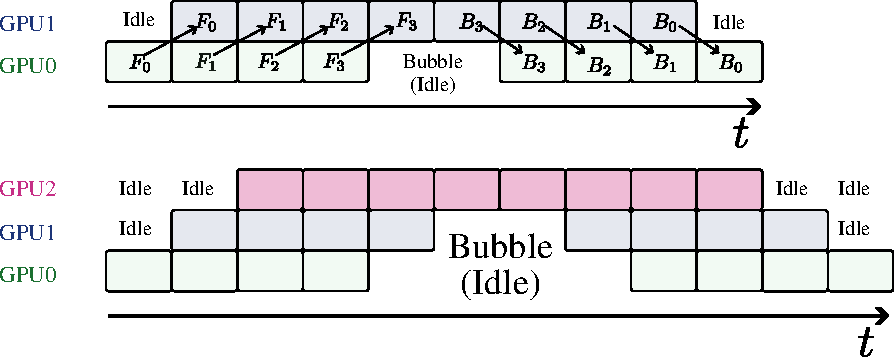
\includegraphics[scale=0.8]{./images/pipeline.pdf}
	\caption{The Illustration of the pipeline parallel on two GPUs. As you can see the bubble tends to grow as we increase the number of GPUs}
\end{figure}

\paragraph{Example:} Imagine a 2-stage pipeline parallel setup (for simplicity):

\begin{itemize}
	\item GPU 0: Holds Layers 1–3  
	\item GPU 1: Holds Layers 4–6  
\end{itemize}

If you have a batch of data with 32 samples, you might split it into 4 micro-batches of size 8 each. Then, forward Pass can be processed as follows:
\begin{enumerate}
	\item Micro-Batch 1
		\begin{enumerate}
			\item Step A: GPU 0 processes layers 1–3 for micro-batch #1.
			\item Step B: Once GPU 0 is done with those layers, it sends the activations for micro-batch #1 over to GPU 1.
			\item Step C: GPU 1 then processes layers 4–6 for micro-batch #1.
		\end{enumerate}
	\item Micro-Batch 2
		\begin{enumerate}
			\item As soon as GPU 0 finishes Step A for micro-batch #1 and passes the data to GPU 1, GPU 0 is free to start micro-batch #2 (layers 1–3).
			\item Meanwhile, GPU 1 is busy processing micro-batch #1 (layers 4–6).
			\item Once GPU 0 finishes its part for micro-batch #2, it sends those activations to GPU 1—which will be ready to handle them as soon as it’s done with micro-batch #1.
		\end{enumerate}
	\item Micro-Batch 3 and 4
		\begin{enumerate}
			\item This pattern continues in an overlapping fashion: while GPU 1 is busy with micro-batch #2, GPU 0 can start on micro-batch #3, and so on.
		\end{enumerate}
\end{enumerate}

The key benefit is concurrency:
\begin{itemize}
	\item While GPU 0 is processing micro-batch 2, GPU 1 can process micro-batch 1.  
	\item This overlap leads to higher GPU utilization.
\end{itemize}

Backward pass is a bit more complex because:
\begin{itemize}
	\item You need gradient signals to flow in the reverse order of the forward pipeline.  
	\item Each stage waits until it receives the gradient from the next stage before it can compute its own local gradients and pass them back to the previous stage.
\end{itemize}

However, the overall concept is similar-multiple stages can run backprop (on different micro-batches) in parallel, thereby keeping all GPUs busy.


\subsection{Pipeline Bubbles}

When using pipeline parallelism, you often hear about \textit{pipeline bubbles}. This refers to idle times on some GPUs before the assembly line is fully loaded or after it starts to wind down. 
\begin{itemize}
	\item Start-up Bubble: In the very beginning, GPU 1 must wait until GPU 0 finishes the first forward pass for micro-batch 1. GPU 1 sits idle during that initial delay.  
	\item Wind-down Bubble: After the last micro-batch enters GPU 0, GPU 1 continues to process the pipeline while GPU 0 is idle.
\end{itemize}

These bubbles can lead to less-than-ideal speedups, but you can mitigate them by using enough micro-batches to keep the pipeline busy most of the time.

\subsection{Combining Pipeline Parallelism with Other Forms of Parallelism}

In practice, pipeline parallelism is often combined with:
\begin{itemize}
	\item Data Parallelism: You still replicate each stage across multiple GPUs to handle separate shards of data.  
	\item Tensor Parallelism / Model Parallelism: Instead of giving entire layers to one GPU, you split the parameters or compute of a single layer across multiple GPUs (common in large language model setups, \eg Megatron-LM).  
	\item Sharded Optimizer Approaches (\eg ZeRO, FSDP): Distribute optimizer states and gradients to reduce memory overhead.
\end{itemize}


\section{1F1B}

\begin{figure}[t]
	\centering
	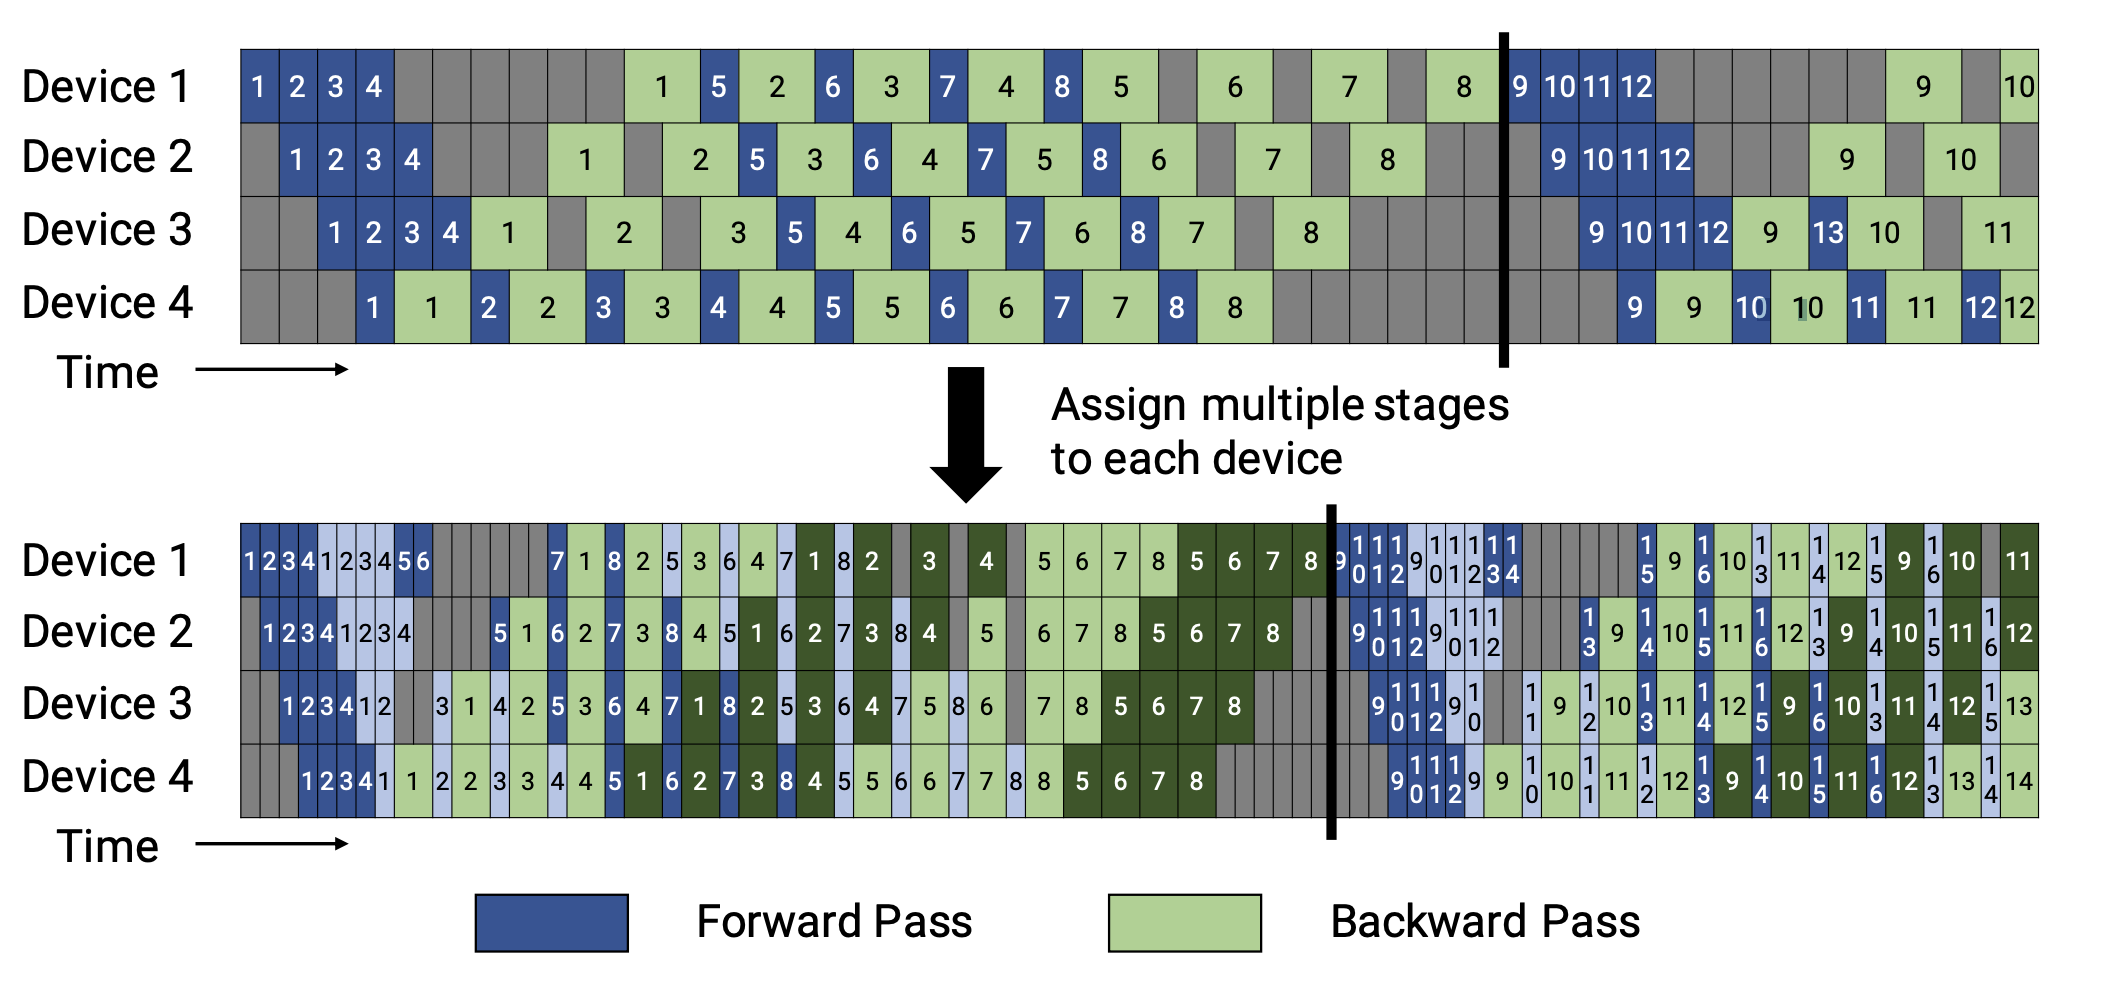
\includegraphics[scale=0.23]{./images/1f1b.png}
\end{figure}

\subsection{Non-interleaved Schedule}

The non-interleaved schedule can be divided into two states. The first state is the startup state (or warm-up state). In the startup state, After completing the forward pass for the first minibatch, it performs the backward pass for the same minibatch, and then starts alternating between performing forward and backward passes for subsequent minibatches. As the backward pass starts propagating to earlier stages in the pipeline, every stage starts alternating between forward and backward pass for different minibatches. As shown in the above figure, in the steady state, every machine is busy either doing the forward pass or backward pass for a minibatch.

\subsection{Interleaved Schedule}

This schedule requires the number of microbatches to be an integer multiple of the stage of pipeline. In this schedule, each device can perform computation for multiple subsets of layers(called a model chunk) instead of a single contiguous set of layers. \ie Before device 1 had layer 1-4; device 2 had layer 5-8; and so on. But now device 1 has layer 1,2,9,10; device 2 has layer 3,4,11,12; and so on. With this scheme, each device in the pipeline is assigned multiple pipeline stages and each pipeline stage has less computation. This mode is both memory-efficient and time-efficient.


\section{Zero Bubble}
\label{sec:}


\part{Transformers}
\chapter{Attention}

Both self-attention and multi-head attention perform similar core operations—projecting inputs into queries, keys, and values; computing dot products; and then combining information—but they do so in slightly different ways. Below, we break down the computational cost for each, using common notation, and then summarize the differences.

---

## Notation and Basic Costs

Let:
- \( n \) be the sequence length.
- \( d \) be the hidden (feature) dimension of each token.
- \( H \) be the number of heads (for multi-head attention).
- \( d_k \) be the dimension of each head’s queries and keys. (Typically, \( d_k = d / H \).)

Two main parts contribute to the computational cost:
1. **Linear projections** that map the input to queries, keys, and values.
2. **Attention score computations and weighted-sum operations** (dominated by matrix multiplications).

---

## 1. Self-Attention (Single-Head)

### A. Linear Projections

For an input \( X \) of shape \((n, d)\), we project it into three matrices:
- \( Q = X W^Q \) with \( W^Q \in \mathbb{R}^{d \times d} \)
- \( K = X W^K \) with \( W^K \in \mathbb{R}^{d \times d} \)
- \( V = X W^V \) with \( W^V \in \mathbb{R}^{d \times d} \)

The cost of each projection is roughly \( O(n \, d \, d) = O(n\, d^2) \). For three projections, the cost is
\[
O(3 \, n\, d^2) \quad \text{(or simply } O(n\, d^2) \text{ up to constants).}
\]

### B. Attention Score Computation

The attention scores are computed as:
\[
\text{Scores} = \frac{QK^\top}{\sqrt{d}}.
\]
- \( Q \) is \( n \times d \) and \( K^\top \) is \( d \times n \), so the matrix multiplication costs \( O(n \, d \, n) = O(n^2\, d) \).

### C. Softmax and Weighted Sum

1. **Softmax over each row:**  
   For each of the \( n \) rows (each of length \( n \)), the cost is \( O(n) \). Over all rows, that’s \( O(n^2) \).  
2. **Weighted Sum:**  
   Multiplying the resulting \( n \times n \) attention matrix with \( V \) (which is \( n \times d \)) also costs \( O(n^2\, d) \).

### D. Total Cost (Self-Attention)

Summing the costs:
- Projections: \( O(n\, d^2) \)
- Dot-product (score) computation: \( O(n^2\, d) \)
- Softmax and weighted sum: \( O(n^2) + O(n^2\, d) \) (the \( O(n^2\, d) \) term dominates when \( d \) is not tiny)

Thus, the total computational cost is:
\[
O(n\, d^2 + n^2\, d).
\]

For long sequences (large \( n \)), the \( O(n^2\, d) \) term (quadratic in \( n \)) is the dominant cost.

---

## 2. Multi-Head Attention

Multi-head attention splits the hidden dimension into \( H \) parts and performs self-attention in parallel over these “heads.” Let’s analyze the cost per head and then sum over all heads.

### A. Linear Projections

For each head \( h \) (where \( h = 1, \dots, H \)), we project the input \( X \) into:
- \( Q^{(h)} = X W_h^Q \) with \( W_h^Q \in \mathbb{R}^{d \times d_k} \)
- \( K^{(h)} = X W_h^K \) with \( W_h^K \in \mathbb{R}^{d \times d_k} \)
- \( V^{(h)} = X W_h^V \) with \( W_h^V \in \mathbb{R}^{d \times d_k} \)

Each projection costs \( O(n \, d\, d_k) \). Since \( d_k = d / H \), the cost per projection per head is
\[
O\Big(n\, d\, \frac{d}{H}\Big) = O\Big(\frac{n\, d^2}{H}\Big).
\]
There are 3 projections per head, so per head cost is \( O(n\, d^2 / H) \). Summing over all \( H \) heads:
\[
O\Big(H \times \frac{n\, d^2}{H}\Big) = O(n\, d^2).
\]

### B. Attention Score Computation per Head

For each head, the attention scores are computed as:
\[
\text{Scores}^{(h)} = \frac{Q^{(h)} \, (K^{(h)})^\top}{\sqrt{d_k}}.
\]
- \( Q^{(h)} \) is \( n \times d_k \) and \( (K^{(h)})^\top \) is \( d_k \times n \), costing \( O(n\, d_k\, n) = O(n^2\, d_k) \).

Since \( d_k = d / H \), the cost per head is:
\[
O\Big(n^2 \frac{d}{H}\Big).
\]
Over all \( H \) heads, the total cost is:
\[
O\Big(H \times n^2\, \frac{d}{H}\Big) = O(n^2\, d).
\]

### C. Softmax and Weighted Sum (per head)

For each head, applying softmax and computing the weighted sum with \( V^{(h)} \) also costs \( O(n^2) \) for softmax plus \( O(n^2\, d_k) \) for the weighted sum. Summing over all heads, the dominant cost remains
\[
O(n^2\, d),
\]
since the softmax operations over \( n \) tokens and \( H \) heads combine to a similar scale as in single-head attention.

### D. Final Linear Projection

After computing the attention outputs for all heads, they are concatenated (forming an \( n \times d \) matrix) and then passed through a final linear projection with cost \( O(n\, d^2) \).

### E. Total Cost (Multi-Head Attention)

Adding everything together:
- Projections into heads: \( O(n\, d^2) \)
- Per-head attention (scores, softmax, weighted sum): \( O(n^2\, d) \)
- Final projection: \( O(n\, d^2) \)

Thus, the overall computational cost is still:
\[
O(n\, d^2 + n^2\, d).
\]

---

## Comparison and Key Points

1. **Quadratic Cost in Sequence Length:**  
   Both self-attention and multi-head attention have a term \( O(n^2\, d) \), which means that as the sequence length \( n \) increases, the cost grows quadratically. This is primarily due to the pairwise dot products between queries and keys.

2. **Linear Projections Cost:**  
   The cost for projecting inputs to queries, keys, and values is \( O(n\, d^2) \). This is common to both single-head and multi-head versions, although multi-head attention splits the projections among heads (but still sums up to the same overall cost).

3. **Parallelization:**  
   Multi-head attention can be parallelized over the \( H \) heads. In practice, this allows hardware (like GPUs) to compute all heads simultaneously, which may improve throughput even though the theoretical number of operations is similar.

4. **Memory Considerations:**  
   Both methods need to store an \( n \times n \) attention matrix (or \( H \) matrices of size \( n \times n \)), so memory usage also scales quadratically with \( n \).

5. **Expressive Power vs. Cost:**  
   While multi-head attention doesn’t reduce the asymptotic cost compared to single-head attention, it tends to improve model performance by allowing the model to attend to information from different representation subspaces.

---

## Summary

- **Self-Attention:**  
  Total cost is \( O(n\, d^2 + n^2\, d) \). The quadratic term \( O(n^2\, d) \) (from computing the \( n \times n \) attention scores) dominates for long sequences.

- **Multi-Head Attention:**  
  Despite splitting into \( H \) heads, the overall cost remains \( O(n\, d^2 + n^2\, d) \) because:
  - Projections across heads still sum to \( O(n\, d^2) \).
  - Each head computes \( O(n^2\, (d/H)) \) work, which summed over \( H \) heads gives \( O(n^2\, d) \).

In both cases, the key computational bottleneck is the quadratic dependency on the sequence length \( n \), which has spurred research into more efficient attention mechanisms for very long sequences.


\section{Multi-Head Attention}
\label{sec:transformer:mha}

In decoder‐only (autoregressive) models like those used in language generation, the self-attention mechanism must be computed sequentially during inference. This setup introduces a few key issues:
\begin{enumerate}
	\item Growing Computational Cost: During inference, the model generates tokens one by one. For each new token, the self-attention mechanism must consider all previously generated tokens. Concretely, if you have generated \( n \) tokens so far, computing self-attention at the next step involves calculating attention over an \( n \)-length sequence. Since the attention operation involves a dot-product between queries and all keys, its computational cost per new token is roughly proportional to \( O(n \cdot d) \) (ignoring the projection costs). Over a long sequence, this means the overall computation grows roughly quadratically with the sequence length \( n \).  
		\begin{itemize}
			\item Example: At time step 1 you compute attention over 1 token, at step 2 over 2 tokens, and so on. By the \( N \)th token, you’re performing operations over \( N \) tokens, leading to a total cost that scales as \( 1 + 2 + \dots + N \sim O(N^2) \).
		\end{itemize}
	\item Increasing Memory Footprint:  Each new token requires storing its associated key and value vectors. As the sequence length grows, the model must maintain larger and larger caches of these vectors. This can become a bottleneck in memory usage, especially for very long generated sequences.

	\item Sequential Dependency and Latency:  Because each token depends on all the previous tokens (via the attention mechanism), you cannot generate multiple tokens in parallel. This inherently sequential process leads to higher latency during inference compared to training, where the full sequence is available and parallelized.
	\item Mitigation via Caching:  
   To reduce repeated computation, many implementations cache the computed keys and values from previous time steps. When generating a new token, the model reuses the cached keys and values rather than recomputing them. While this helps avoid redundant work, the attention computation still scales with the growing length of the cached sequence, and managing this cache can add complexity (both in terms of memory management and in ensuring efficient access).
\end{enumerate}



---

### Summary

- **Quadratic Complexity:** Each new token’s attention calculation involves all past tokens, resulting in a cumulative \( O(n^2) \) cost as the sequence grows.
- **Memory Growth:** The cache for key/value vectors grows linearly with the sequence length.
- **Sequential Generation:** Autoregressive generation forces a sequential process that can be slow compared to parallel operations during training.

These issues are at the heart of why researchers are exploring more efficient attention mechanisms (like sparse attention or linearized attention) for handling long sequences during inference.







A **Transformer** layer uses *multi-head attention* to let each “head” attend to different positions in the input sequence, potentially capturing different relationships and patterns. Specifically:

1. You have an input sequence of \(n\) tokens, each represented as a vector of size \(d_{\text{model}}\).
2. You create **Queries (Q)**, **Keys (K)**, and **Values (V)** from those inputs via learned linear transformations.
3. Instead of having just one set of Q, K, V (i.e., “one head”), you split the embedding dimension \(d_{\text{model}}\) into multiple smaller “heads” and apply scaled dot-product attention in parallel.
4. You then **concatenate** the results of all heads and apply another linear transformation to produce the final output.

---

## Sources of Inefficiency

1. **Quadratic Complexity in Sequence Length (\(O(n^2)\))**  
   - For each attention head, you compute a score matrix \(\mathbf{Q}\mathbf{K}^T\) that is of size \(n \times n\).  
   - This grows quadratically with the sequence length \(n\).  

2. **Overhead from Multiple Heads**  
   - Each head has its own Q, K, V matrices and does a separate dot-product and softmax operation. Even if each head works with a smaller dimension (e.g., \(d_{\text{model}} / h\)), you still do these computations \(h\) times.  

3. **Memory Footprint**  
   - Storing these intermediate score matrices and outputs for backpropagation can become very large. For \(B\) batches of length \(n\) and \(h\) heads, the attention scores alone can occupy a \((B \times h \times n \times n)\) tensor in memory.  

4. **Redundancy Among Heads**  
   - Empirically, some heads may learn very similar attention patterns or “do nothing” important, which can waste parameters and computation.  

---

## A Simple Example

Let’s consider a toy sequence of **4 tokens**, each of dimension **8** (i.e., \(n = 4\), \(d_{\text{model}} = 8\)):

\[
\text{Sequence} = [\text{Token}_1, \text{Token}_2, \text{Token}_3, \text{Token}_4]
\]
Each token \(\text{Token}_i\) is a vector in \(\mathbb{R}^8\), for example:  
\[
\text{Token}_1 = [0.2,\; -1.0,\; 0.3,\; 2.1,\; \ldots,\; 0.7].
\]

### Case 1: Single-Head Attention
If we had **single-head** attention (not split into multiple heads):

1. **Compute Q, K, and V**:  
   - We have three weight matrices, each of size \(8 \times 8\) (because \(d_{\text{model}} = 8\)).  
   - For each of the 4 tokens, we apply these transformations:
     \[
     \mathbf{Q}_i = \mathbf{W}^Q \times \text{Token}_i, \quad
     \mathbf{K}_i = \mathbf{W}^K \times \text{Token}_i, \quad
     \mathbf{V}_i = \mathbf{W}^V \times \text{Token}_i.
     \]
     Each \(\mathbf{Q}_i, \mathbf{K}_i, \mathbf{V}_i\) is an 8-dimensional vector.

2. **Compute Attention Scores \(\mathbf{Q}\mathbf{K}^T\)**:  
   - \(\mathbf{Q}\) is a \(4 \times 8\) matrix (all queries stacked).  
   - \(\mathbf{K}\) is a \(4 \times 8\) matrix (all keys stacked).  
   - The product \(\mathbf{Q} \mathbf{K}^T\) is a \(4 \times 4\) matrix (\(n \times n\)).  

3. **Apply Softmax and Multiply by \(\mathbf{V}\)**:  
   - We get attention weights (a \(4 \times 4\) matrix).  
   - Multiply these weights by a \(4 \times 8\) \(\mathbf{V}\)-matrix to get the final output for this single head.

In total, we have one \(4 \times 4\) attention matrix, plus the overhead of storing intermediate transformations.

### Case 2: Two-Head Attention
Now we split the dimension \(d_{\text{model}}=8\) into **2 heads** each of dimension \(4\) (\(d_{\text{head}} = 8/2 = 4\)).

1. **Compute Q, K, and V** for each head separately:  
   - Instead of a single \(\mathbf{W}^Q\) of shape \(8 \times 8\), we now have two sets of parameters:  
     - \(\mathbf{W}^Q_{\text{head1}}\): \(8 \times 4\)  
     - \(\mathbf{W}^Q_{\text{head2}}\): \(8 \times 4\)  
   - Similarly for \(\mathbf{W}^K\) and \(\mathbf{W}^V\) for head 1 and head 2.  
   - For each token, we produce \((\mathbf{Q}_1, \mathbf{K}_1, \mathbf{V}_1)\) for head 1 and \((\mathbf{Q}_2, \mathbf{K}_2, \mathbf{V}_2)\) for head 2.  
   - Now, each \(\mathbf{Q}_1\) is a 4-dimensional vector, and each \(\mathbf{Q}_2\) is also 4-dimensional, etc.

2. **Compute Attention for Each Head**:  
   - For head 1: \(\mathbf{Q}_1\mathbf{K}_1^T\) is \(4 \times 4\).  
   - For head 2: \(\mathbf{Q}_2\mathbf{K}_2^T\) is \(4 \times 4\).  

   We get two separate \(4 \times 4\) score matrices.

3. **Concatenate & Project**:  
   - Each head produces an output of shape \(4 \times 4\) (because we multiply a \(4 \times 4\) attention matrix by a \(4 \times 4\) \(\mathbf{V}\) matrix).  
   - We then **concatenate** these two “4D outputs” (head 1 and head 2) into an 8D vector per token.  
   - Finally, we apply an extra linear projection \(\mathbf{W}^O\) (typically \(8 \times 8\)) to get the final 8D output for each of the 4 tokens.

**Result**:  
- We compute **two** separate attention matrices (\(4 \times 4\) each).  
- We have to store them in memory, perform two sets of softmax, and maintain two sets of Q, K, V parameters.  
- Compared to the single-head scenario, we do effectively twice the attention scoring steps, though each step is at half the embedding dimension.  
- In practice, the overhead is not necessarily “half + half = the same.” There are added overheads from dealing with multiple sets of weights, memory layout, etc.

### How the Inefficiency Grows
- If we scale from \(n=4\) to \(n=1000\) (a relatively short text document), the **attention score matrix** is \(1000 \times 1000\) = **1 million** entries per head.  
- With \(h=12\) heads (typical in a small Transformer), you have \(12\) million attention scores in **one layer**. Large Transformers can have dozens of layers.  
- Each step must also keep track of gradients for backpropagation, so memory usage multiplies.

---

## Putting It All Together

1. **Quadratic Growth in \(n\)**:  
   - Even with a small dimension like 8 or 16, computing a \(n \times n\) attention matrix quickly becomes expensive for large \(n\).  

2. **Multiple Heads Add Overhead**:  
   - Splitting into more heads means repeated Q, K, V transformations, repeated matrix multiplications, repeated softmax operations, and more storage of intermediate results.

3. **Memory Footprint**:  
   - Especially during training, we need to keep the attention weights and intermediate activations for **each head** for backward pass.  
   - This is \(\mathcal{O}(B \times h \times n^2)\) in memory, where \(B\) is batch size, \(h\) is number of heads, and \(n\) is sequence length.

4. **Redundant Heads**:  
   - Empirically, not all heads are unique or helpful. Some might learn nearly identical patterns, leading to parameter inefficiency.  

### Why Do We Still Use Multi-Head Attention?
- **Powerful Representation**: Multiple heads allow the model to attend to different aspects of the sequence simultaneously (e.g., one head might focus on local context, another on distant context).  
- **Empirical Success**: Despite the inefficiencies, multi-head attention consistently leads to state-of-the-art results in NLP, and it is used in widely popular models like BERT, GPT, T5, etc.  

---

## Strategies to Mitigate Inefficiency

1. **Sparse or Limited Attention**:  
   - Replace full \(n \times n\) attention with sparse patterns (e.g., Longformer, Big Bird, Reformer), reducing complexity from \(O(n^2)\) to something like \(O(n)\) or \(O(n \log n)\).

2. **Linear Attention**:  
   - Use kernels or approximations (Performer, Linear Transformers) so you never explicitly compute the \(\mathbf{Q}\mathbf{K}^T\) matrix.

3. **Memory-Efficient Implementations**:  
   - Techniques like **FlashAttention** compute attention with minimal intermediate storage on GPUs.

4. **Pruning or Tying Heads**:  
   - **Pruning**: Remove heads that contribute little to model performance.  
   - **Parameter sharing**: Use the same projection matrices across heads or layers to reduce parameters.

---

## In Summary

- **Multi-head attention** is powerful but **inefficient** primarily due to its \(O(n^2)\) complexity in sequence length, compounded by overhead from multiple heads.  
- Even with a small toy example (4 tokens, 2 heads), you can see how the computations and intermediate matrices multiply.  
- In real-world scenarios with thousands of tokens, the memory and compute costs become substantial.  
- **Despite** these inefficiencies, multi-head attention remains widely used because it **empirically works extremely well** and has become a cornerstone of modern deep learning architectures for language, vision, and beyond.


\section{KV Caching}
\label{sec:transformer:kv_caching}

In transformer-based language models—especially those that generate text one token at a time, such as GPT-style models—**key-value caching** is a technique used at inference (decoding) time to avoid recomputing attention over all previously generated tokens. Below is an explanation of how it works and the mathematical underpinnings.

---

## 1. Background: Multi-Head Attention Recap

A transformer block uses multi-head attention. Let:

- \(X \in \mathbb{R}^{T \times d_\text{model}}\) be the sequence of input embeddings at a given layer (where \(T\) is sequence length and \(d_\text{model}\) is the hidden dimension).
- We compute three matrices (for each head) from \(X\):
  \[
  Q = XW^Q,\quad
  K = XW^K,\quad
  V = XW^V
  \]
  where \(W^Q, W^K, W^V \in \mathbb{R}^{d_\text{model} \times d_k}\). In multi-head attention, we do this for \(h\) heads and then combine results.

- The standard scaled dot-product attention for one head is:
  \[
  \text{Attention}(Q, K, V) 
  = \text{softmax}\!\Bigl(\frac{QK^T}{\sqrt{d_k}}\Bigr)\, V.
  \]

- For a single self-attention head in the decoder, when autoregressively generating token \(t\), the query corresponds to the current token’s hidden state, while \(K\) and \(V\) come from **all** previously generated tokens (including the current one, depending on the exact indexing).

---

## 2. Autoregressive Decoding Without Caching

In an autoregressive setup:
1. We generate the first token, then feed it back into the model to generate the second.
2. We then feed the first two tokens to generate the third, and so on.

Naively, each step would require re-running the entire attention stack over all tokens generated so far. For instance, at step \(t\), you would compute:
\[
K_{1:t},\ V_{1:t},\ \text{and } Q_t,
\]
from the first \(t\) tokens. This is computationally expensive because for each new token, all \(K_{1:t}\) and \(V_{1:t}\) have to be re-derived from scratch.

---

## 3. Key-Value Caching

### 3.1. High-Level Idea

To avoid re-computing \(K_{1:t}\) and \(V_{1:t}\) at each new time step, we **cache** them from previous steps. That is, once you have computed \(K_{1:t}\) and \(V_{1:t}\) at step \(t\), you can store them (in “cache”). When you move to step \(t+1\), you only need to compute the *new* \(K_{t+1}\) and \(V_{t+1}\) (i.e., the keys and values for the newly generated token), then **concatenate** them to the cached keys and values:
\[
\begin{aligned}
K_{1:t+1} &= \bigl[K_{1:t},\, K_{t+1}\bigr], \\
V_{1:t+1} &= \bigl[V_{1:t},\, V_{t+1}\bigr].
\end{aligned}
\]
Hence, the next attention step becomes:
\[
\text{Attention}\bigl(Q_{t+1}, K_{1:t+1}, V_{1:t+1}\bigr).
\]

Crucially, we do **not** need to recompute \(K_{1:t}\) and \(V_{1:t}\) from scratch because they are already cached.

### 3.2. Detailed Math

Let’s formalize this in the context of a single head (multi-head is just a repetition over heads):

1. **At time step \(t\)** (generating the \(t\)-th token):
   - Input hidden state for time step \(t\) (just a single token’s embedding in the decoder) is \(x_t \in \mathbb{R}^{1 \times d_\text{model}}\).
   - We compute:
     \[
     Q_t = x_t\, W^Q, \quad
     K_t = x_t\, W^K, \quad
     V_t = x_t\, W^V.
     \]
   - The shape of each (assuming batch size 1 for simplicity) is \(\mathbb{R}^{1 \times d_k}\).
   
2. **Caching**:  
   Suppose at step \(t-1\), we had already cached:
   \[
   K_{1:t-1} \in \mathbb{R}^{(t-1) \times d_k}, \quad
   V_{1:t-1} \in \mathbb{R}^{(t-1) \times d_k}.
   \]
   We now build:
   \[
   K_{1:t} = 
   \begin{pmatrix}
   K_{1:t-1}\\ 
   K_t
   \end{pmatrix}, \quad
   V_{1:t} = 
   \begin{pmatrix}
   V_{1:t-1}\\ 
   V_t
   \end{pmatrix}.
   \]
   This concatenation along the time dimension yields new shapes:
   \[
   K_{1:t} \in \mathbb{R}^{t \times d_k}, \quad
   V_{1:t} \in \mathbb{R}^{t \times d_k}.
   \]

3. **Attention at step \(t\)**:
   \[
   \text{Attention}(Q_t, K_{1:t}, V_{1:t}) 
   \;=\; \mathrm{softmax}\!\Bigl(\frac{Q_t \, K_{1:t}^T}{\sqrt{d_k}}\Bigr)\, V_{1:t}.
   \]
   Here, 
   - \(Q_t K_{1:t}^T \in \mathbb{R}^{1 \times t}\),  
   - \(\mathrm{softmax}\) is applied along the last dimension,  
   - Final result is \(\mathbb{R}^{1 \times d_k}\).

4. **Repeat for step \(t+1\)**:
   - Compute \(Q_{t+1}, K_{t+1}, V_{t+1}\).  
   - Append (cache):
     \[
     K_{1:t+1} = \bigl[K_{1:t};\, K_{t+1}\bigr], \quad
     V_{1:t+1} = \bigl[V_{1:t};\, V_{t+1}\bigr].
     \]
   - Then:
     \[
     \text{Attention}(Q_{t+1}, K_{1:t+1}, V_{1:t+1})
     = \mathrm{softmax}\!\Bigl(\frac{Q_{t+1} \, K_{1:t+1}^T}{\sqrt{d_k}}\Bigr)\, V_{1:t+1}.
     \]

By *caching* \(K_{1:t}\) and \(V_{1:t}\), the model does not recalculate them from the entire sequence at every generation step. Instead, it just concatenates the newly computed \(K_t\) and \(V_t\).

---

## 4. Shapes and Practical Considerations

When dealing with batch sizes, multiple heads, and GPU-friendly shapes, the cached keys and values typically have shapes like:

- **During inference** (for a batch of size \(B\) and \(h\) heads):
  \[
  K \in \mathbb{R}^{B \times h \times T \times d_k}, \quad
  V \in \mathbb{R}^{B \times h \times T \times d_k}.
  \]
  - \(T\) grows one token at a time in autoregressive generation.  
  - We keep these in GPU memory to make repeated attention operations efficient.

- **Attention** for each head becomes:
  \[
  \mathrm{softmax}\!\Bigl(\frac{Q \times K^T}{\sqrt{d_k}}\Bigr)\, V,
  \]
  where
  \[
  Q \in \mathbb{R}^{B \times h \times 1 \times d_k}, \quad
  K^T \in \mathbb{R}^{B \times h \times d_k \times T}.
  \]
  So the attention logit matrix is \(\mathbb{R}^{B \times h \times 1 \times T}\).

---

## 5. Why Is Key-Value Caching Important?

- **Efficiency**:  
  - Without caching, each step of generation must feed the entire partial sequence \(\{x_1, \ldots, x_t\}\) through all attention layers, resulting in \(\mathcal{O}(t)\) computations per token. Doing that for each of the \(t\) tokens leads to \(\mathcal{O}(t^2)\) complexity for generating \(t\) tokens.
  - With caching, the complexity for each new token is \(\mathcal{O}(1)\) on the transformer's forward pass for the new key/value (plus the cost of computing attention of dimension \(\mathcal{O}(t)\) for the new query). Overall, this significantly speeds up autoregressive decoding.

- **Scalability**:  
  - Large language models often generate hundreds or thousands of tokens in one inference pass. Key-value caching makes real-time or near real-time generation feasible.

---

## 6. Summary

1. **Transformer Self-Attention** relies on queries \((Q)\), keys \((K)\), and values \((V)\).
2. **Autoregressive Decoding** reuses previously generated tokens at each new step.
3. **Key-Value Caching** stores \(K_{1:t}\) and \(V_{1:t}\) in memory so that the model only needs to:
   - Compute the new query \(Q_t\), key \(K_t\), and value \(V_t\) for the latest token,
   - Concatenate them to the cached vectors,
   - Perform the attention with the *already computed* keys and values from previous steps.

Mathematically, for each head \(h\), step \(t\), we have:

\[
\begin{aligned}
&K_{1:t} = [K_{1:t-1};\, K_t], 
\quad
V_{1:t} = [V_{1:t-1};\, V_t], \\[6pt]
&\hat{h}_t = 
\mathrm{softmax}\!\Bigl(\frac{Q_t K_{1:t}^T}{\sqrt{d_k}}\Bigr)\, V_{1:t},
\end{aligned}
\]
where \(\hat{h}_t\) is the attention output for step \(t\). This caching approach is *vital* for efficient large-scale generation in GPT-like models.


\section{Flash Attention}
\label{sec:transformer:flash_attention}

\chapter{Positional Embeddings}
\label{ch:transformer:posemb}

Rather than focusing on a token's absolute position in a sentence, relative positional embeddings concentrate on the distances between pairs of tokens. This method doesn't add a position vector to the word vector directly. Instead, it alters the attention mechanism to incorporate relative positional information.

\subsection{Rotary Positional Embeddings}
RoPE represents a novel approach in encoding positional information. Traditional methods, either absolute or relative, come with their limitations. Absolute positional embeddings assign a unique vector to each position, which though straightforward, doesn't scale well and fails to capture relative positions effectively. Relative embeddings, on the other hand, focus on the distance between tokens, enhancing the model’s understanding of token relationships but complicating the model architecture.

RoPE ingeniously combines the strengths of both. It encodes positional information in a way that allows the model to understand both the absolute position of tokens and their relative distances. This is achieved through a rotational mechanism, where each position in the sequence is represented by a rotation in the embedding space. The elegance of RoPE lies in its simplicity and efficiency, enabling models to better grasp the nuances of language syntax and semantics.

RoPE introduces a novel concept. Instead of adding a positional vector, it applies a rotation to the word vector. Imagine a two-dimensional word vector for ``dog.'' To encode its position in a sentence, RoPE rotates this vector. The angle of rotation ($\theta$) is proportional to the word's position in the sentence. For instance, the vector is rotated by $\theta$ for the first position, $2\theta$ for the second, and so on. This approach has several benefits:

% **Rotary Positional Embeddings (RoPE)** are a method of encoding positional information for tokens in a sequence, commonly used in transformer-based language models. Unlike standard absolute or relative positional embeddings, RoPE encodes positions by *rotating* the token representations in a continuous, differentiable manner that depends on the token’s position index. This rotation imparts position-dependent phase information into the hidden representations.

## 1. Motivation for Positional Embeddings

In transformers, self-attention modules do not have an inherent sense of the order of tokens in a sequence. Hence, we need to inject positional information into the token representations. Various strategies have been developed:

1. **Absolute Positional Embeddings** (Vaswani et al., 2017)  
   \- Add a sinusoidal or learned vector to each token embedding depending on its position index \( i \).  

2. **Relative Positional Embeddings** (Shaw et al., 2018)  
   \- Use position *differences* between tokens to modify attention scores.

3. **Rotary Positional Embeddings (RoPE)** (Su et al., 2021, also popularized in models like GPT-3, LLaMA, etc.)  
   \- Impose a position-dependent *rotation* of the token embedding vectors, yielding a smooth, continuous positional dependence, and enabling better generalization (including, in some cases, extrapolation to sequences longer than those used in training).

---

## 2. Intuition Behind RoPE

RoPE introduces position information by rotating the query and key vectors in each attention head by a position-specific angle. Each pair \((2k, 2k+1)\) of embedding dimensions corresponds to a 2D plane in which a rotation is applied. As the position index \(i\) changes, the rotation angle changes accordingly.

This technique ensures:
- The *relative* positions between tokens manifest as *relative phase* shifts in the query and key representations.
- The attention mechanism can more naturally capture relationships across positions, potentially facilitating better handling of longer sequences.

---

## 3. Mathematical Formulation

Let:
- \( \mathbf{x}_i \in \mathbb{R}^d \) be the embedding vector (for either query \(Q\) or key \(K\)) at position \(i\).
- We partition \(\mathbf{x}_i\) into \(d/2\) “complex” components or 2D planes.  
  Concretely, we can view \(\mathbf{x}_i\) as \(\{ (x_{i,2k}, x_{i,2k+1}) : k = 0, 1, \ldots, \frac{d}{2}-1 \}\).

We define a rotation angle \(\theta_{i, k}\) for each pair of dimensions \((2k, 2k+1)\). One common choice is:

\[
\theta_{i, k} \;=\; i \cdot \alpha_k,
\]

where \(\alpha_k\) might be a scaling based on the dimension index \(k\). A popular definition (akin to sinusoidal absolute embeddings) sets:

\[
\alpha_k \;=\; \frac{1}{10000^{\frac{2k}{d}}}.
\]

### 3.1. Rotation in a 2D Subspace

For each pair \((2k, 2k+1)\), define the rotary transformation \(\text{RoPE}(\cdot)\) as follows. Let

\[
\mathbf{x}_i^{(k)} 
= \begin{pmatrix}
x_{i, 2k} \\[6pt]
x_{i, 2k+1}
\end{pmatrix}.
\]

Then,

\[
\text{RoPE}_i \bigl(\mathbf{x}_i^{(k)}\bigr)
= \begin{pmatrix}
\cos(\theta_{i, k}) & -\sin(\theta_{i, k}) \\
\sin(\theta_{i, k}) & \cos(\theta_{i, k})
\end{pmatrix}
\begin{pmatrix}
x_{i, 2k} \\[4pt]
x_{i, 2k+1}
\end{pmatrix}.
\]

Hence, the updated 2D coordinates are:

\[
\begin{aligned}
\tilde{x}_{i, 2k} &= x_{i, 2k}\,\cos(\theta_{i,k}) \;-\; x_{i, 2k+1}\,\sin(\theta_{i,k}),\\[6pt]
\tilde{x}_{i, 2k+1} &= x_{i, 2k+1}\,\cos(\theta_{i,k}) \;+\; x_{i, 2k}\,\sin(\theta_{i,k}).
\end{aligned}
\]

We perform this rotation across all \(k = 0, 1, \dots, \frac{d}{2}-1\), concatenating the results back into a \(d\)-dimensional vector \(\tilde{\mathbf{x}}_i\).

### 3.2. Applying RoPE to Queries and Keys

In many implementations, we apply RoPE to both the query \(\mathbf{q}_i\) and key \(\mathbf{k}_j\) vectors for each position \(i, j\). That is:

\[
\begin{aligned}
\tilde{\mathbf{q}}_i &= \text{RoPE}_i(\mathbf{q}_i), \\
\tilde{\mathbf{k}}_j &= \text{RoPE}_j(\mathbf{k}_j).
\end{aligned}
\]

Then, during the attention calculation:
\[
\text{Attention}(i, j) 
= \frac{\tilde{\mathbf{q}}_i \,\cdot\, \tilde{\mathbf{k}}_j}{\sqrt{d}}.
\]

The key property is that

\[
\tilde{\mathbf{q}}_i^\top \, \tilde{\mathbf{k}}_j
\;\;=\;\;
\mathbf{q}_i^\top\, \mathbf{M}(i,j)\, \mathbf{k}_j,
\]

where \(\mathbf{M}(i,j)\) is a matrix encoding the position difference \((i-j)\). This yields a relative-positional effect *without* explicitly storing or adding embedding vectors for each position pair.

---

## 4. Key Properties and Advantages

1. **Relative Position Encoding**:  
   Despite being “rotary” in nature, RoPE effectively gives you a *relative* position signal, because the dot product \(\tilde{\mathbf{q}}_i \cdot \tilde{\mathbf{k}}_j\) depends on \(\theta_{i} - \theta_{j}\).

2. **Extrapolation to Longer Sequences**:  
   Because the rotational formulation is continuous in \(i\), there are scenarios (and certain hyperparameter choices) where models can handle positions beyond the training context length more gracefully than standard absolute embeddings.

3. **Parameter Efficiency**:  
   Like sinusoidal absolute embeddings, RoPE can be implemented without adding learnable parameters for each position. The rotation angles \(\theta_{i,k}\) can be defined by a simple function of \(i\) and \(k\).

4. **Smoothness**:  
   The rotation changes smoothly with position index \(i\), which can help the model capture long-range dependencies in a continuous manner.

---

## 5. Practical Implementation Notes

1. **Dimension Splitting**:  
   Typically, the hidden dimension \(d\) for each attention head is split into \(\frac{d}{2}\) rotation “planes.” If \(d\) is not even, one might handle the leftover dimension or pad it to make it even.

2. **Choice of Base**:  
   The base (like 10000) in \(\alpha_k = 1/10000^{2k/d}\) can vary. Some implementations use different scaling constants to adapt to different maximum context lengths.

3. **Software Implementation**:  
   - In frameworks like PyTorch or JAX, one can build a rotation matrix or directly apply the sine/cosine expansions for each pair of channels.  
   - Some models (e.g., GPT-NeoX, LLaMA) treat RoPE as a custom “bias” or “transformation” step in the attention layer.

4. **Extrapolation Tricks**:  
   When aiming to extrapolate beyond the training context, people sometimes rescale the angles \(\theta_{i,k}\) so that the same “maximum angle” used in training applies to larger sequence lengths at inference time.

---

## 6. Relation to Other Position Encoding Methods

- **Absolute Sinusoidal** (from the original Transformer) uses a fixed \(\sin(\cdot)\), \(\cos(\cdot)\) per dimension and position, but it doesn’t rotate the hidden states themselves; instead, it *adds* or *concatenates* these values to the token embeddings.  
- **Learned Absolute** typically uses a trainable embedding table of size `[max_length, hidden_dim]`.  
- **Relative Position Bias** or **Relative Position Embeddings** (Shaw et al.) incorporate \(|i-j|\) or \(i-j\) in a learned or parameterized manner, often adding a bias to the attention logits.  
- **Alibi** (Press et al., 2022) modifies the attention logits with a position-dependent linear bias, which also helps with extrapolation.  

Compared to the above, **RoPE** is lightweight and elegantly encodes relative position effects via a rotation in the embedding space.

---

## 7. Summary

**Rotary Positional Embeddings (RoPE)** introduce a continuous, position-dependent rotation to query/key vectors in attention layers. Each pair of embedding dimensions is treated as a 2D plane in which we apply a rotation matrix whose angle depends on the token’s position index. This approach effectively captures relative position information, can help the model handle longer sequences, and does not require large per-position embedding tables. The key insight is that differences in position become differences in rotation phase, which modifies the dot-product attention in a manner analogous to relative positional embeddings.

---

### References

1. **Vaswani et al.**: “Attention Is All You Need.” *NeurIPS 2017*.  
2. **Su et al. (RoFormer paper)**: “RoFormer: Enhanced Transformer by Rotary Position Embedding.” *arXiv:2104.09864, 2021*.  
3. **Shaw et al.**: “Self-Attention with Relative Position Representations.” *NAACL 2018*.  
4. **Press et al.**: “Train Short, Test Long: Attention with Linear Biases Enables Input Length Extrapolation.” *arXiv:2108.12409, 2021*.  

---

**In essence**, RoPE leverages a simple yet powerful idea: use a rotation in each 2D subspace of the embedding vectors to encode position. This mathematically elegant solution yields strong empirical performance and can be implemented with minimal overhead in modern transformer architectures.



\chapter{Tokenization}
\label{ch:transformer:tokenization}

\chapter{Model Compression}
\label{ch:transformer:compression}



\part{Compression}
\chapter{Model Compression}
\section{Introduction}
haha




\backmatter
% bibliography, glossary and index would go here.

\nocite{*}
\bibliographystyle{unsrt}
\bibliography{references}
\end{document}
